\chapter{Übersicht über die Funktionen von LaTeX}

\section{Introduction}
Hier steht interessanter Text mit Quelle. \cite{example_citation} \todo{hier ist ein TODO} Mehr toller Text. Damit die Quelle beim Text bleibt verwende ich das (siehe editor): ~\cite{example_citation} 
Ich kann auch Abkürzungen verwenden: \ac{ki} ist ein nützliches Tool, wenn ich Fragen zu LaTeX habe. Mit \ac{ki} kann ich vieles lernen.

\subsection{Hier eine Unterüberschrift}
Mehr interessante Informationen. Lorem ipsum dolor sit amet, consetetur sadipscing elitr, sed diam nonumy eirmod tempor invidunt ut labore et dolore magna aliquyam erat, sed diam voluptua. At vero eos et accusam et justo duo dolores et ea rebum. Stet clita kasd gubergren, no sea takimata sanctus est Lorem ipsum dolor sit amet. Lorem ipsum dolor sit amet, consetetur sadipscing elitr, sed diam nonumy eirmod tempor invidunt ut labore et dolore magna aliquyam erat, sed diam voluptua. At vero eos et accusam et justo duo dolores et ea rebum. Stet clita kasd gubergren, no sea takimata sanctus est Lorem ipsum dolor sit amet. \todo[inline]{Hier ein inline TODO}

\section{Bilder}

Ich kann Bilder so einfügen:
\begin{figure}[h]
    \centering
    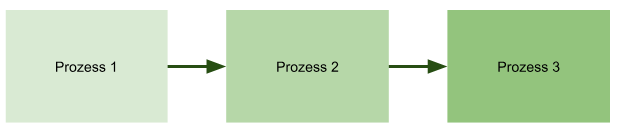
\includegraphics[width=0.5\linewidth]{figures/Beispiel_Bild.png}
    \caption{Quelle klebt am Text: ~\cite{example_citation}}
    \label{fig:Beipsielbild}
\end{figure}



\section{Listen}
\begin{enumerate}[label=\arabic*.]
    \item Nudeln
    \item Gemüse
    \begin{enumerate}[label=\arabic{enumi}.\arabic*.]
        \item Paprika
        \item Karotten
    \end{enumerate}
    \item Pesto
\end{enumerate}

\section{Tabellen}
\begin{table}[H]
    \centering
    \begin{tabular}[H]{l|l|l}
        Bezeichnung & Füße& Schnäbel\\
        \hline
        Ente& 2& 1\\
        \hline
        Katze& 4& 0\\
    \end{tabular}
    \caption{Tiere}
\end{table}


\section{Quellcode}
\begin{lstlisting}[language=java, caption=Hello World in Java, captionpos=b]
    class HelloWorld {
        public static void main(String[] args) {
            System.out.println("Hello World!");
        }
    }
\end{lstlisting}

Manuell ins Inhaltsverzeichnis eingefügte Überschrift (siehe Editor)
\addcontentsline{toc}{section}{Manuell ins Inhaltsverzeichnis eingefügte Überschrift}

\section*{Diese Section wird nicht im Inhaltsverzeichnis angezeigt} %geht auch mit \chapter oder \subsection
